\chapter{Measurements of Charge Transfer Efficiency in the SNIFS Detectors}

\section{Introduction}
Traps in the silicon lattice of the CCD can capture charge and release it at a later time. The trapped and released charge can result in smearing of point sources along the direction of charge transfer and can impede our ability to get accurate photon counts. To understand this effect, we measure the charge transfer efficiency (CTE) of the CCDs. The CTE of a CCD is the fraction of charge that survives each pixel transfer. Because CCDs used in astronomical applications make many transfers in each image, the CTE must be very close to unity, with typical values being around $1-10^{-6}$.

Because a larger number of transfers results in a higher likelihood of encountering more traps, pixels that are further from the readout register are more effected by trapped charge. This effect is especially problematic for spectroscopic instruments like SNIFS since the increased smearing with distance to the amplifier can lead to uneven broadening of spectral features.

Our goal was to quantify the charge transfer efficiency in all channels (photometric, and blue and red spectroscopic) of SNIFS using two methods. The initial characterization was done by first exposing the CCDs to a Fe-55 x-ray source to generate single-pixel events with a known spectrum and then measuring the photo-electron loss along the readout. Later, in-situ measurements were enabled by performing a similar analysis using cosmic ray events extracted from the dark frames taken during each observing run.

\section{Initial Characterization with Fe-55 X-rays}
A simple way of measuring the charge transfer efficiency of a CCD is to expose the chip to photons of a known energy. Each resulting hit on the CCD results in a known amount of charge being generated in the event. By plotting the amount of charge measured in each event vs the row number, we can see if the amount of charge that is read out decreases with increasing distance to the amplifier (a sign that the charge is being trapped along the way) and quantify this trapping.

We performed this experiment by exposing each CCD to a Fe-55 X-ray source. Fe-55 has a strong lines from K-alpha and K-beta emission at 5.9 keV and 6.2 keV, corresponding to signals in the CCD of about 1620 $\textrm{e}^-$ and 1778 $\textrm{e}^-$, respectively. Using \verb|SExtractor|, we selected all events that were 5$\sigma$ above the background. We calculated the gain, $g$, in each individual frame by fitting two Gaussians to the spectrum of fluxes, $s(f)$, extracted from these events.

\begin{equation}
    s = A_1 \exp\left(-\frac{(f-1620/g)^2}{2\sigma_1^2}\right) + A_2 \exp\left(-\frac{(f-1778/g)^2}{2\sigma_2^2}\right)
\end{equation}

\begin{figure}
    \centering
    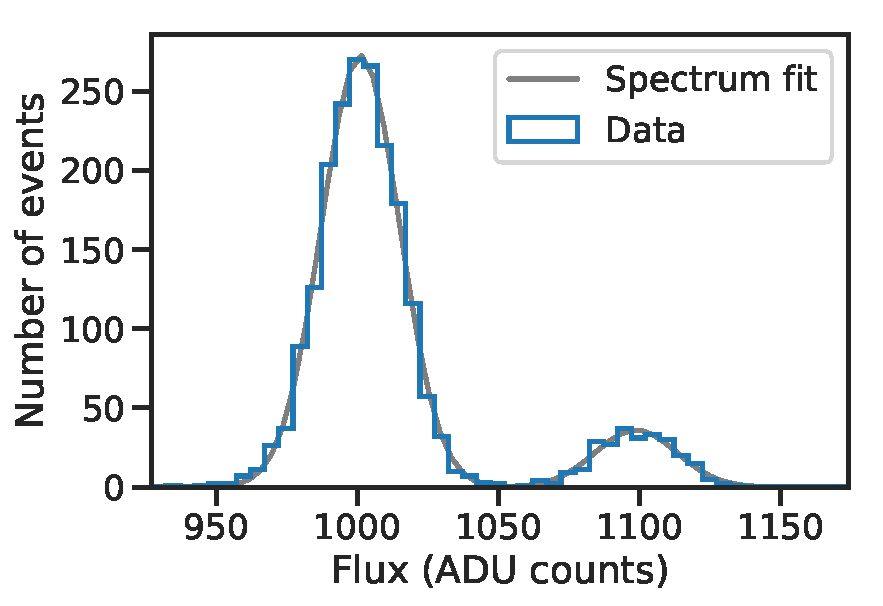
\includegraphics{figures/cte/spectrum_fit.pdf}
    \caption{Example spectrum of X-ray hit events extracted from a single exposure. The histogram of ADU counts per event is shown in blue, and the best fit K-alpha and K-beta emission lines are shown in gray.}
    \label{fig:xray_spectrum}
\end{figure}

Combining the events from several X-ray frames (22 for the blue channel, 26 for the red channel, and 8 for the photometric channel), we plotted the flux for each event as a function of distance from the amplifier. By fitting a line to the data points corresponding to the K-alpha emission, we can measure how much charge is lost per transfer by dividing the slope (in units of $e^-$ per transfer) by the total number of electrons expected (1620).

The scatter plots of number of electrons vs. number of serial register transfers and number of parallel register transfers are shown in Figs. \ref{fig:cte_xray} and \ref{fig:cte_xray_serial} respectively. The resulting measurements of the charge transfer efficiency are found in Table \ref{tab:cte_xray}.

\begin{figure}
    \centering
    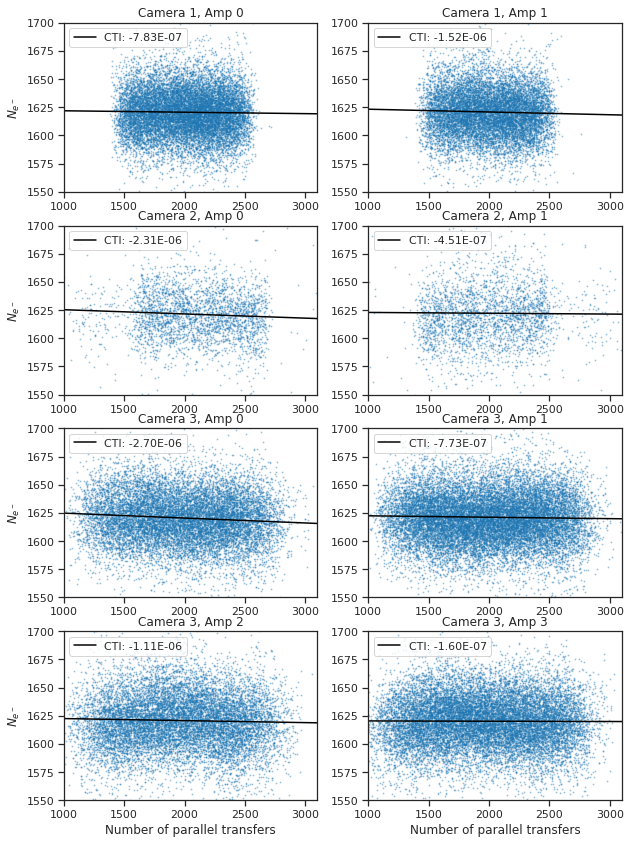
\includegraphics[width=0.9\textwidth]{figures/cte/xray_cte_parallel.png}
    \caption{Number of electrons measured in K-alpha emission line as a function of number of parallel register transfers for each amplifier in each CCD. The best-fit line is shown in black with the legend indicating the slope, which measures the charge-transfer inefficiency.}
    \label{fig:cte_xray}
\end{figure}

\begin{figure}
    \centering
    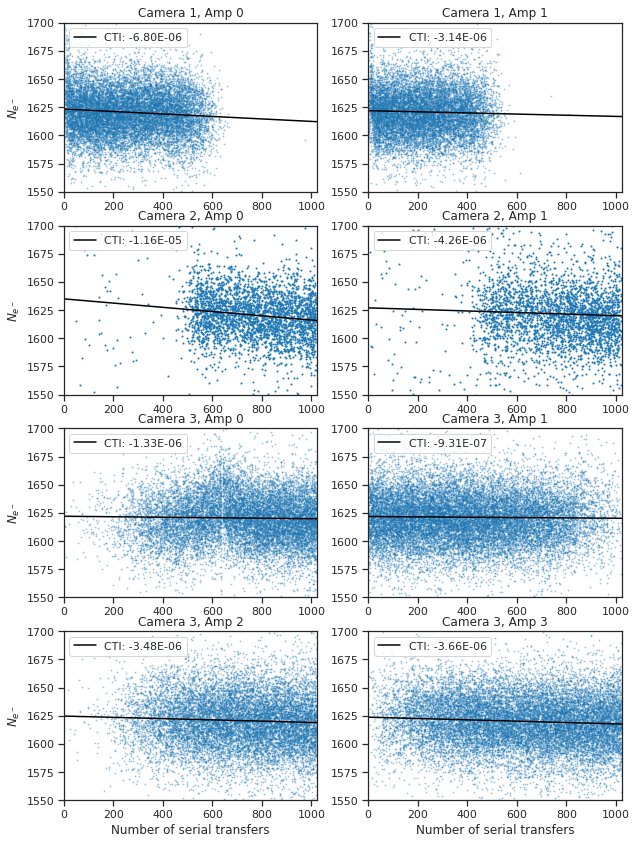
\includegraphics[width=0.9\textwidth]{figures/cte/xray_cte_serial.png}
    \caption{Same as \ref{fig:cte_xray}, but for serial register transfers rather than parallel register transfers.}
    \label{fig:cte_xray_serial}
\end{figure}

\begin{table}[]
    \centering
    \begin{tabular}{|c|c|c|c|c|c|}\hline
        Camera & Amp. & Parallel CTI & Serial CTI & Number of frames & Number of hits \\\hline
        B & A &0.783 $\;\pm\;$ 0.015 & 6.80 $\;\pm\;$ 0.03 & 22 & 15,925 \\
          & B &1.519 $\;\pm\;$ 0.017 & 3.14 $\;\pm\;$ 0.03 &    & 13,113 \\\hline
        R & A &2.312 $\;\pm\;$ 0.016 & 11.60 $\;\pm\;$ 0.04 & 26 & 4,071 \\
          & B &0.451 $\;\pm\;$ 0.011 & 4.26 $\;\pm\;$ 0.03 &    & 4,415 \\\hline
        P & A &2.696 $\;\pm\;$ 0.010 & 1.33 $\;\pm\;$ 0.02 & 8 & 15,308 \\
          & B &0.773 $\;\pm\;$ 0.008 & 0.93 $\;\pm\;$ 0.01 &   & 21,010 \\
          & C &1.109 $\;\pm\;$ 0.009 & 3.48 $\;\pm\;$ 0.02 &   & 14,498 \\
          & D &0.160 $\;\pm\;$ 0.008 & 3.66 $\;\pm\;$ 0.01 &   & 19,041 \\\hline
    \end{tabular}
    \caption{Charge transfer efficiency results from Fe-55 X-ray characterization. All values are in units of $10^{-6}$.}
    \label{tab:cte_xray}
\end{table}

\section{Cosmic Ray Measurement}
The X-ray measurement allows for a precise determination of the CTI if we have access to the detector. However, we'd like to be able to track changes in the CTI with time to see if there is any degradation over the course of the instrument lifetime.

By using cosmic ray hits found in dark frames, we can get an \emph{in-situ} measurement of the charge transfer efficiency on a nightly basis. 

Cosmic rays hits in the CCD do not all have the same energy, so we cannot perform the exact same analysis as we did for the X-ray tests. However, we can take advantage of the fact that charge transfer inefficiency causes smearing along the line of charge transfer along with the fact that the magnitude of this smearing increase with distance from the amplifier.

Our process is as follows:

\begin{itemize}
    \item For each dark frame taken, use \verb|SExtractor| to find cosmic ray hits. Cosmic ray hits are defined as the objects detected 1.5$\sigma$ over the noise, with a measured ellipticity $<$ 0.2 and no flags raised. Example hits are shown in Fig. \ref{fig:example_hits}. In order to avoid the noise potentially introduced by hits landing in the CTI trails of other nearby hits (see e.g. the bottom right example in Fig. \ref{fig:example_hits}), we remove from our sample all pairs of hits that are within 10 pixels of each other.
    
    \item For each cosmic ray hit, we subtract the value of the pixels above the peak (i.e. further from the readout amplifier) from the pixels below the peak. On average, this will remove the symmetric components (from oblique incidence angles and charge diffusion in the bulk silicon) from the average cosmic ray hits, leaving only the CTI trails.
    
    \item We calculate the fraction of charge in the trail by summing the number of excess counts in the 5 trailing pixels and divide it by the number of counts in the peak of the hit
    
    \item By plotting the median fraction of charge lost to CTI as a function of distance from the readout amplifier and fit a line to the data. The slope of the line gives us a measure of the charge transfer inefficiency.
    
\end{itemize}

\begin{figure}
    \centering
    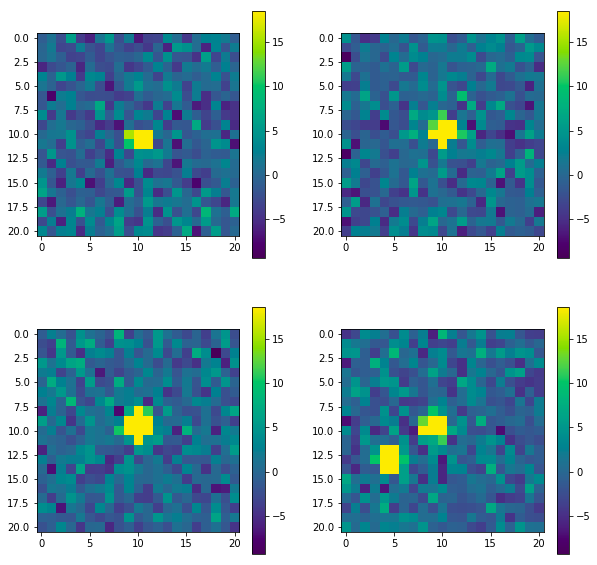
\includegraphics[width=0.9\textwidth]{figures/cte/example_hits.png}
    \caption{Example identified cosmic ray hits passing our ellipticity cut. The two neighboring hits seen in the bottom right example would be removed from the final sample because they are too close to each other. This culling removes some of the noise from our final signal.}
    \label{fig:example_hits}
\end{figure}

We aggregate these measurements on a nightly basis. Fig. \ref{fig:cte_single_night} shows the fraction of counts lost to CTE as a function of distance to the amplifier in each amplifier for a single night.

\begin{figure}
    \centering
    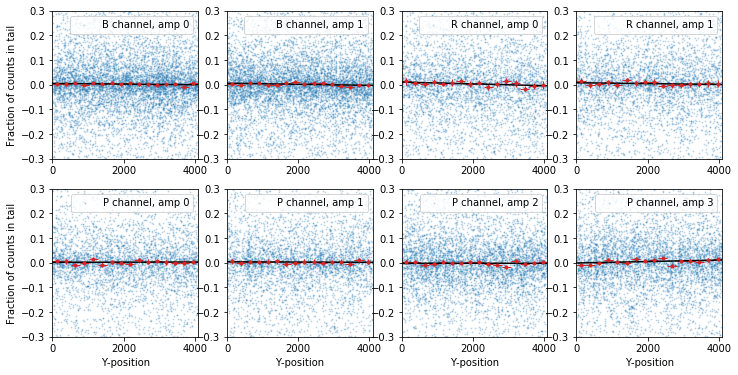
\includegraphics[width=0.9\textwidth]{figures/cte/single_night_example_parallel.png}
    \caption{Example measurement of CTI from cosmic ray tails from a single night. All blue dots represent a single cosmic ray hit. The red points show the median fraction of counts in the peak of the hits to end up in the tails in each y-position bin. The best-fit line is also shown. The slope of this line gives us the CTI.}
    \label{fig:cte_single_night}
\end{figure}

We repeat these measurements for every night in order to check for time dependence. In Fig. \ref{fig:time_variation} we show the CTI as a function of time for each amplifier. There is very little evidence of significant degradation over time.

\begin{figure}
    \centering
    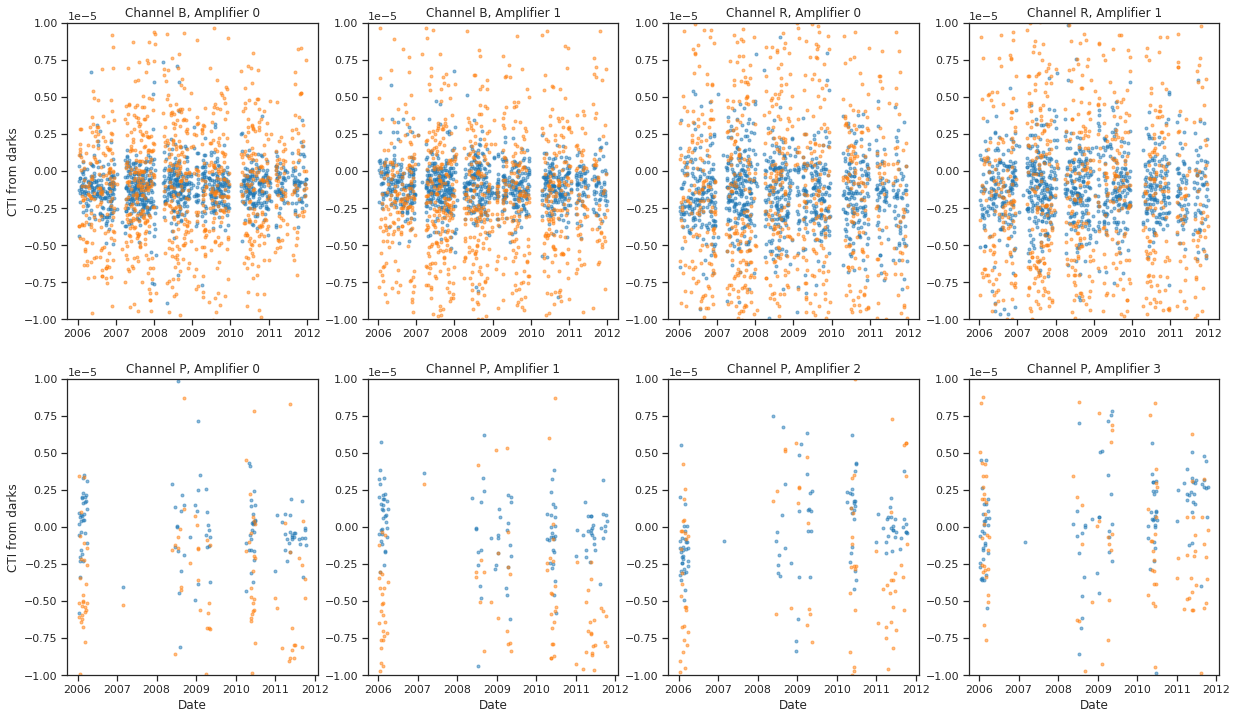
\includegraphics[width=0.9\textwidth]{figures/cte/time_variation.png}
    \caption{A search for potential time variation in the charge transfer efficiency of each of the spectroscopic cameras. No time variation is visible.}
    \label{fig:time_variation}
\end{figure}

The average CTI numbers for each amplifier are summarized in Table \ref{tab:cte_darks}.
\begin{table}[h!]
    \centering
    \begin{tabular}{|c|c|c|c|}\hline
        Camera & Amplifier & Median Parallel CTI  & Median Serial CTI \\ \hline
        B & A &   1.08 $\pm$ 0.04  &  0.96 $\pm$ 0.13 \\
          & B &   0.97 $\pm$ 0.04  &  2.02 $\pm$ 0.13 \\\hline
        R & A &   1.49 $\pm$ 0.07  &  2.4  $\pm$ 0.2 \\
          & B &   1.24 $\pm$ 0.07  &  2.3  $\pm$ 0.2 \\\hline
        P & A &   0.19 $\pm$ 0.18  &  5.1  $\pm$ 0.5 \\
          & B &   0.18 $\pm$ 0.19  &  7.0  $\pm$ 0.4 \\
          & C &   0.3  $\pm$ 0.2   &  5.4  $\pm$ 0.7 \\
          & D &   0.5  $\pm$ 0.2   &  1.9  $\pm$ 0.5 \\\hline
    \end{tabular}
    \caption{Distribution of CTI measurements over time from all dark frames collected from 2006 to 2012.}
    \label{tab:cte_darks}
\end{table}

% \begin{deluxetable}{lcD@{$\ \pm\ $}DD@{$\ \pm\ $}Dcl}
% \tablecolumns{8}
% \tablecaption{Spectroscopic Channel Detector Charge Transfer Inefficiency}
% \tablehead{
% \colhead{Channel}        &
% \colhead{Amp}            &
% \multicolumn2c{Parallel} &
% \multicolumn2c{Serial}   &
% \colhead{N}              &
% \colhead{Method \&}      &
% \colhead{}               &
% \colhead{}               &
% \multicolumn2c{CTI}      &
% \multicolumn2c{CTI}      &
% \colhead{}               &
% \colhead{Source}        }
% \decimals
% \startdata
% B        &  A  &   0.17 & 0.29  &   1.13 & 0.64  & 22   & Fe$^{55}$ slop\\
%          &     &  0.783 & 0.015 &   6.80 & 0.03  & 22   & Fe$^{55}$ SD\\
%          &     &  1.085 & 0.035 &   0.97 & 0.13  & 1008 & Cosmic rays\\[0.5em]
%          &  B  &   1.37 & 0.37  &   1.42 & 0.95  & 22   & Fe$^{55}$ slop\\
%          &     &  1.519 & 0.017 &   3.14 & 0.03  & 22   & Fe$^{55}$ SD\\
%          &     &   0.98 & 0.04  &   2.02 & 0.13  & 1008 & Cosmic rays\\[1em]
% R        &  A  &   0.54 & 0.73  &  25.30 & 2.57  & 12   & Fe$^{55}$ slop \\
%          &     &   3    & 0.5   &   6    & 0.5   & 1    & Fe$^{55}$ E2V\\
%          &     & 2.312  & 0.016 & 11.60  & 0.04  & 26   & Fe$^{55}$ SD\\
%          &     &  1.49  & 0.07  & 2.4    & 0.2   & 991  & Cosmic rays\\[0.5em]
%          &  B  &  -1.01 & 0.66  & -26.78 & 2.23  & 12   & Fe$^{55}$ slop\\
%          &     &   3    & 0.5   &   7    & 0.5   & 1    & Fe$^{55}$ E2V\\
%          &     &  0.451 & 0.011 & 4.26   & 0.03  & 26   & Fe$^{55}$ SD\\
%          &     & 1.24   & 0.07  & 2.3    & 0.2   & 991  & Cosmic rays\\[0.5em]
% \enddata
% \tablecomments{All CTI values are in units of $10^{-6}$.}
% \end{deluxetable}
% \begin{deluxetable}{lcD@{$\ \pm\ $}DD@{$\ \pm\ $}Dcl}
% \tablecolumns{8}
% \tablecaption{Photometric Channel Detector Charge Transfer Inefficiency}
% \tablehead{
% \colhead{Channel}        &
% \colhead{Amp}            &
% \multicolumn2c{Parallel} &
% \multicolumn2c{Serial}   &
% \colhead{N}              &
% \colhead{Method \&}      &
% \colhead{}               &
% \colhead{}               &
% \multicolumn2c{CTI}      &
% \multicolumn2c{CTI}      &
% \colhead{}               &
% \colhead{Source}        }
% \decimals
% \startdata
% P imager &  A  &   0.31 & 0.13  &   7.38 & 0.20  & 34   & Fe$^{55}$ slop\\
%          &     &   0    & 0.5   &   7    & 0.5   & 34   & Fe$^{55}$ E2V\\
%          &     & 2.696  & 0.010 & 1.33   & 0.02  & 8    & Fe$^{55}$ SD\\
%          &     & 0.19   & 0.18  & 5.1    & 0.5   & 119  & Cosmic rays\\
%          &  B  &   0.20 & 0.08  &  -8.17 & 0.15  & 34   & Fe$^{55}$ slop\\
%          &     &   0    & 0.5   &   8    & 0.5   &  1   & Fe$^{55}$ E2V\\
%          &     & 0.773  & 0.008 & 3.48   & 0.02  & 8    & Fe$^{55}$ SD\\
%          &     & 0.18   & 0.19  &  7.0   & 0.4   & 119  & Cosmic rays\\
% P guider &  A  &  -0.40 & 0.11  &   5.70 & 0.20  & 34   & Fe$^{55}$ slop\\
%          &     &   1    & 0.5   &   3    & 0.5   &  1   & Fe$^{55}$ E2V\\
%          &     & 1.109  & 0.009 & 3.48   & 0.02  & 8    & Fe$^{55}$ SD\\
%          &     &  0.3   & 0.2   & 5.4    & 0.2   & 119  & Cosmic rays\\
%          &  B  &  -0.10 & 0.10  &  -2.66 & 0.16  & 34   & Fe$^{55}$ slop\\
%          &     &   1    & 0.5   &   4    & 0.5   &  1   & Fe$^{55}$ E2V\\
%          &     & 0.160  & 0.008 & 3.55   & 0.01  & 8    & Fe$^{55}$ SD\\
%          &     &  0.5   & 0.3   & 1.9    & 0.5   & 119  & Cosmic rays\\\\
% \enddata
% \tablecomments{All CTI values are in units of $10^{-6}$.}
% \end{deluxetable}
